% Created by tikzDevice version 0.10.1 on 2019-04-10 16:42:59
% !TEX encoding = UTF-8 Unicode
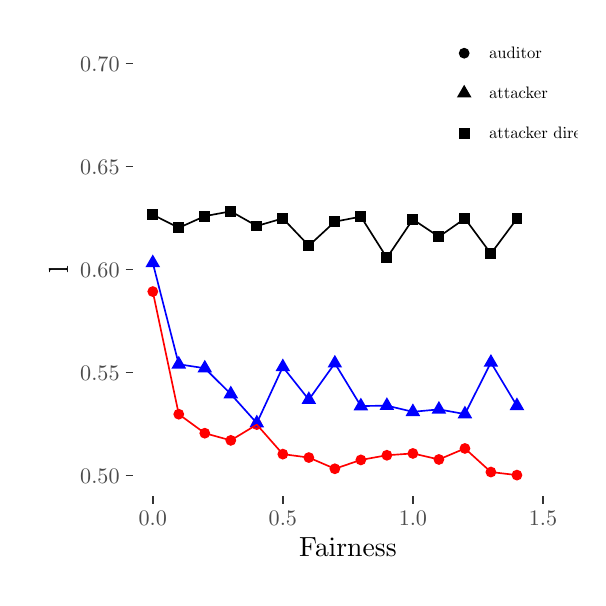
\begin{tikzpicture}[x=1pt,y=1pt]
\definecolor{fillColor}{RGB}{255,255,255}
\path[use as bounding box,fill=fillColor,fill opacity=0.00] (0,0) rectangle (198.74,198.74);
\begin{scope}
\path[clip] (  0.00,  0.00) rectangle (198.74,198.74);
\definecolor{drawColor}{RGB}{255,255,255}
\definecolor{fillColor}{RGB}{255,255,255}

\path[draw=drawColor,line width= 0.6pt,line join=round,line cap=round,fill=fillColor] ( -0.00,  0.00) rectangle (198.74,198.74);
\end{scope}
\begin{scope}
\path[clip] ( 38.16, 29.45) rectangle (193.24,193.24);
\definecolor{fillColor}{RGB}{255,0,0}

\path[fill=fillColor] ( 45.21,103.38) circle (  1.96);
\definecolor{fillColor}{RGB}{0,0,255}

\path[fill=fillColor] ( 45.21,116.79) --
	( 47.85,112.21) --
	( 42.56,112.21) --
	cycle;
\definecolor{fillColor}{RGB}{0,0,0}

\path[fill=fillColor] ( 43.24,129.20) --
	( 47.17,129.20) --
	( 47.17,133.13) --
	( 43.24,133.13) --
	cycle;
\definecolor{fillColor}{RGB}{255,0,0}

\path[fill=fillColor] ( 54.60, 59.07) circle (  1.96);
\definecolor{fillColor}{RGB}{0,0,255}

\path[fill=fillColor] ( 54.60, 80.16) --
	( 57.25, 75.58) --
	( 51.96, 75.58) --
	cycle;
\definecolor{fillColor}{RGB}{0,0,0}

\path[fill=fillColor] ( 52.64,124.45) --
	( 56.57,124.45) --
	( 56.57,128.38) --
	( 52.64,128.38) --
	cycle;
\definecolor{fillColor}{RGB}{255,0,0}

\path[fill=fillColor] ( 64.00, 52.20) circle (  1.96);
\definecolor{fillColor}{RGB}{0,0,255}

\path[fill=fillColor] ( 64.00, 78.73) --
	( 66.65, 74.16) --
	( 61.36, 74.16) --
	cycle;
\definecolor{fillColor}{RGB}{0,0,0}

\path[fill=fillColor] ( 62.04,128.68) --
	( 65.97,128.68) --
	( 65.97,132.60) --
	( 62.04,132.60) --
	cycle;
\definecolor{fillColor}{RGB}{255,0,0}

\path[fill=fillColor] ( 73.40, 49.61) circle (  1.96);
\definecolor{fillColor}{RGB}{0,0,255}

\path[fill=fillColor] ( 73.40, 69.40) --
	( 76.05, 64.82) --
	( 70.76, 64.82) --
	cycle;
\definecolor{fillColor}{RGB}{0,0,0}

\path[fill=fillColor] ( 71.44,130.41) --
	( 75.37,130.41) --
	( 75.37,134.34) --
	( 71.44,134.34) --
	cycle;
\definecolor{fillColor}{RGB}{255,0,0}

\path[fill=fillColor] ( 82.80, 55.31) circle (  1.96);
\definecolor{fillColor}{RGB}{0,0,255}

\path[fill=fillColor] ( 82.80, 58.90) --
	( 85.44, 54.33) --
	( 80.16, 54.33) --
	cycle;
\definecolor{fillColor}{RGB}{0,0,0}

\path[fill=fillColor] ( 80.84,125.12) --
	( 84.76,125.12) --
	( 84.76,129.04) --
	( 80.84,129.04) --
	cycle;
\definecolor{fillColor}{RGB}{255,0,0}

\path[fill=fillColor] ( 92.20, 44.64) circle (  1.96);
\definecolor{fillColor}{RGB}{0,0,255}

\path[fill=fillColor] ( 92.20, 79.21) --
	( 94.84, 74.63) --
	( 89.56, 74.63) --
	cycle;
\definecolor{fillColor}{RGB}{0,0,0}

\path[fill=fillColor] ( 90.24,127.85) --
	( 94.16,127.85) --
	( 94.16,131.78) --
	( 90.24,131.78) --
	cycle;
\definecolor{fillColor}{RGB}{255,0,0}

\path[fill=fillColor] (101.60, 43.40) circle (  1.96);
\definecolor{fillColor}{RGB}{0,0,255}

\path[fill=fillColor] (101.60, 67.37) --
	(104.24, 62.79) --
	( 98.96, 62.79) --
	cycle;
\definecolor{fillColor}{RGB}{0,0,0}

\path[fill=fillColor] ( 99.64,118.00) --
	(103.56,118.00) --
	(103.56,121.92) --
	( 99.64,121.92) --
	cycle;
\definecolor{fillColor}{RGB}{255,0,0}

\path[fill=fillColor] (111.00, 39.35) circle (  1.96);
\definecolor{fillColor}{RGB}{0,0,255}

\path[fill=fillColor] (111.00, 80.52) --
	(113.64, 75.95) --
	(108.36, 75.95) --
	cycle;
\definecolor{fillColor}{RGB}{0,0,0}

\path[fill=fillColor] (109.04,126.68) --
	(112.96,126.68) --
	(112.96,130.61) --
	(109.04,130.61) --
	cycle;
\definecolor{fillColor}{RGB}{255,0,0}

\path[fill=fillColor] (120.40, 42.55) circle (  1.96);
\definecolor{fillColor}{RGB}{0,0,255}

\path[fill=fillColor] (120.40, 65.06) --
	(123.04, 60.49) --
	(117.76, 60.49) --
	cycle;
\definecolor{fillColor}{RGB}{0,0,0}

\path[fill=fillColor] (118.44,128.50) --
	(122.36,128.50) --
	(122.36,132.42) --
	(118.44,132.42) --
	cycle;
\definecolor{fillColor}{RGB}{255,0,0}

\path[fill=fillColor] (129.80, 44.23) circle (  1.96);
\definecolor{fillColor}{RGB}{0,0,255}

\path[fill=fillColor] (129.80, 65.21) --
	(132.44, 60.63) --
	(127.16, 60.63) --
	cycle;
\definecolor{fillColor}{RGB}{0,0,0}

\path[fill=fillColor] (127.84,113.62) --
	(131.76,113.62) --
	(131.76,117.54) --
	(127.84,117.54) --
	cycle;
\definecolor{fillColor}{RGB}{255,0,0}

\path[fill=fillColor] (139.20, 44.89) circle (  1.96);
\definecolor{fillColor}{RGB}{0,0,255}

\path[fill=fillColor] (139.20, 62.98) --
	(141.84, 58.41) --
	(136.55, 58.41) --
	cycle;
\definecolor{fillColor}{RGB}{0,0,0}

\path[fill=fillColor] (137.24,127.51) --
	(141.16,127.51) --
	(141.16,131.43) --
	(137.24,131.43) --
	cycle;
\definecolor{fillColor}{RGB}{255,0,0}

\path[fill=fillColor] (148.60, 42.71) circle (  1.96);
\definecolor{fillColor}{RGB}{0,0,255}

\path[fill=fillColor] (148.60, 63.86) --
	(151.24, 59.28) --
	(145.95, 59.28) --
	cycle;
\definecolor{fillColor}{RGB}{0,0,0}

\path[fill=fillColor] (146.63,121.22) --
	(150.56,121.22) --
	(150.56,125.14) --
	(146.63,125.14) --
	cycle;
\definecolor{fillColor}{RGB}{255,0,0}

\path[fill=fillColor] (158.00, 46.69) circle (  1.96);
\definecolor{fillColor}{RGB}{0,0,255}

\path[fill=fillColor] (158.00, 62.16) --
	(160.64, 57.58) --
	(155.35, 57.58) --
	cycle;
\definecolor{fillColor}{RGB}{0,0,0}

\path[fill=fillColor] (156.03,127.81) --
	(159.96,127.81) --
	(159.96,131.73) --
	(156.03,131.73) --
	cycle;
\definecolor{fillColor}{RGB}{255,0,0}

\path[fill=fillColor] (167.39, 38.17) circle (  1.96);
\definecolor{fillColor}{RGB}{0,0,255}

\path[fill=fillColor] (167.39, 80.80) --
	(170.04, 76.22) --
	(164.75, 76.22) --
	cycle;
\definecolor{fillColor}{RGB}{0,0,0}

\path[fill=fillColor] (165.43,115.11) --
	(169.36,115.11) --
	(169.36,119.03) --
	(165.43,119.03) --
	cycle;
\definecolor{fillColor}{RGB}{255,0,0}

\path[fill=fillColor] (176.79, 37.06) circle (  1.96);
\definecolor{fillColor}{RGB}{0,0,255}

\path[fill=fillColor] (176.79, 65.14) --
	(179.44, 60.56) --
	(174.15, 60.56) --
	cycle;
\definecolor{fillColor}{RGB}{0,0,0}

\path[fill=fillColor] (174.83,127.76) --
	(178.76,127.76) --
	(178.76,131.69) --
	(174.83,131.69) --
	cycle;
\definecolor{drawColor}{RGB}{255,0,0}

\path[draw=drawColor,line width= 0.6pt,line join=round] ( 45.21,103.38) --
	( 54.60, 59.07) --
	( 64.00, 52.20) --
	( 73.40, 49.61) --
	( 82.80, 55.31) --
	( 92.20, 44.64) --
	(101.60, 43.40) --
	(111.00, 39.35) --
	(120.40, 42.55) --
	(129.80, 44.23) --
	(139.20, 44.89) --
	(148.60, 42.71) --
	(158.00, 46.69) --
	(167.39, 38.17) --
	(176.79, 37.06);
\definecolor{drawColor}{RGB}{0,0,255}

\path[draw=drawColor,line width= 0.6pt,line join=round] ( 45.21,113.74) --
	( 54.60, 77.11) --
	( 64.00, 75.68) --
	( 73.40, 66.35) --
	( 82.80, 55.85) --
	( 92.20, 76.16) --
	(101.60, 64.32) --
	(111.00, 77.47) --
	(120.40, 62.01) --
	(129.80, 62.16) --
	(139.20, 59.93) --
	(148.60, 60.81) --
	(158.00, 59.11) --
	(167.39, 77.75) --
	(176.79, 62.09);
\definecolor{drawColor}{RGB}{0,0,0}

\path[draw=drawColor,line width= 0.6pt,line join=round] ( 45.21,131.17) --
	( 54.60,126.41) --
	( 64.00,130.64) --
	( 73.40,132.37) --
	( 82.80,127.08) --
	( 92.20,129.82) --
	(101.60,119.96) --
	(111.00,128.64) --
	(120.40,130.46) --
	(129.80,115.58) --
	(139.20,129.47) --
	(148.60,123.18) --
	(158.00,129.77) --
	(167.39,117.07) --
	(176.79,129.72);
\end{scope}
\begin{scope}
\path[clip] (  0.00,  0.00) rectangle (198.74,198.74);
\definecolor{drawColor}{gray}{0.30}

\node[text=drawColor,anchor=base east,inner sep=0pt, outer sep=0pt, scale=  0.80] at ( 33.21, 34.14) {0.50};

\node[text=drawColor,anchor=base east,inner sep=0pt, outer sep=0pt, scale=  0.80] at ( 33.21, 71.36) {0.55};

\node[text=drawColor,anchor=base east,inner sep=0pt, outer sep=0pt, scale=  0.80] at ( 33.21,108.59) {0.60};

\node[text=drawColor,anchor=base east,inner sep=0pt, outer sep=0pt, scale=  0.80] at ( 33.21,145.82) {0.65};

\node[text=drawColor,anchor=base east,inner sep=0pt, outer sep=0pt, scale=  0.80] at ( 33.21,183.04) {0.70};
\end{scope}
\begin{scope}
\path[clip] (  0.00,  0.00) rectangle (198.74,198.74);
\definecolor{drawColor}{gray}{0.20}

\path[draw=drawColor,line width= 0.6pt,line join=round] ( 35.41, 36.89) --
	( 38.16, 36.89);

\path[draw=drawColor,line width= 0.6pt,line join=round] ( 35.41, 74.12) --
	( 38.16, 74.12);

\path[draw=drawColor,line width= 0.6pt,line join=round] ( 35.41,111.34) --
	( 38.16,111.34);

\path[draw=drawColor,line width= 0.6pt,line join=round] ( 35.41,148.57) --
	( 38.16,148.57);

\path[draw=drawColor,line width= 0.6pt,line join=round] ( 35.41,185.80) --
	( 38.16,185.80);
\end{scope}
\begin{scope}
\path[clip] (  0.00,  0.00) rectangle (198.74,198.74);
\definecolor{drawColor}{gray}{0.20}

\path[draw=drawColor,line width= 0.6pt,line join=round] ( 45.21, 26.70) --
	( 45.21, 29.45);

\path[draw=drawColor,line width= 0.6pt,line join=round] ( 92.20, 26.70) --
	( 92.20, 29.45);

\path[draw=drawColor,line width= 0.6pt,line join=round] (139.20, 26.70) --
	(139.20, 29.45);

\path[draw=drawColor,line width= 0.6pt,line join=round] (186.19, 26.70) --
	(186.19, 29.45);
\end{scope}
\begin{scope}
\path[clip] (  0.00,  0.00) rectangle (198.74,198.74);
\definecolor{drawColor}{gray}{0.30}

\node[text=drawColor,anchor=base,inner sep=0pt, outer sep=0pt, scale=  0.80] at ( 45.21, 18.99) {0.0};

\node[text=drawColor,anchor=base,inner sep=0pt, outer sep=0pt, scale=  0.80] at ( 92.20, 18.99) {0.5};

\node[text=drawColor,anchor=base,inner sep=0pt, outer sep=0pt, scale=  0.80] at (139.20, 18.99) {1.0};

\node[text=drawColor,anchor=base,inner sep=0pt, outer sep=0pt, scale=  0.80] at (186.19, 18.99) {1.5};
\end{scope}
\begin{scope}
\path[clip] (  0.00,  0.00) rectangle (198.74,198.74);
\definecolor{drawColor}{RGB}{0,0,0}

\node[text=drawColor,anchor=base,inner sep=0pt, outer sep=0pt, scale=  1.00] at (115.70,  7.70) {Fairness};
\end{scope}
\begin{scope}
\path[clip] (  0.00,  0.00) rectangle (198.74,198.74);
\definecolor{drawColor}{RGB}{0,0,0}

\node[text=drawColor,rotate= 90.00,anchor=base,inner sep=0pt, outer sep=0pt, scale=  1.00] at ( 14.59,111.34) {l};
\end{scope}
\begin{scope}
\path[clip] (  0.00,  0.00) rectangle (198.74,198.74);
\definecolor{fillColor}{RGB}{255,255,255}

\path[fill=fillColor] (146.24,149.11) rectangle (209.23,204.62);
\end{scope}
\begin{scope}
\path[clip] (  0.00,  0.00) rectangle (198.74,198.74);
\definecolor{fillColor}{RGB}{0,0,0}

\path[fill=fillColor] (157.73,189.51) circle (  1.96);
\end{scope}
\begin{scope}
\path[clip] (  0.00,  0.00) rectangle (198.74,198.74);
\definecolor{fillColor}{RGB}{0,0,0}

\path[fill=fillColor] (157.73,178.11) --
	(160.38,173.53) --
	(155.09,173.53) --
	cycle;
\end{scope}
\begin{scope}
\path[clip] (  0.00,  0.00) rectangle (198.74,198.74);
\definecolor{fillColor}{RGB}{0,0,0}

\path[fill=fillColor] (155.77,158.64) --
	(159.70,158.64) --
	(159.70,162.56) --
	(155.77,162.56) --
	cycle;
\end{scope}
\begin{scope}
\path[clip] (  0.00,  0.00) rectangle (198.74,198.74);
\definecolor{drawColor}{RGB}{0,0,0}

\node[text=drawColor,anchor=base west,inner sep=0pt, outer sep=0pt, scale=  0.60] at (166.77,187.44) {auditor};
\end{scope}
\begin{scope}
\path[clip] (  0.00,  0.00) rectangle (198.74,198.74);
\definecolor{drawColor}{RGB}{0,0,0}

\node[text=drawColor,anchor=base west,inner sep=0pt, outer sep=0pt, scale=  0.60] at (166.77,172.99) {attacker};
\end{scope}
\begin{scope}
\path[clip] (  0.00,  0.00) rectangle (198.74,198.74);
\definecolor{drawColor}{RGB}{0,0,0}

\node[text=drawColor,anchor=base west,inner sep=0pt, outer sep=0pt, scale=  0.60] at (166.77,158.54) {attacker direct};
\end{scope}
\end{tikzpicture}
